% Parte III: Questões específicas do problema de N-corpos
% - Como lidar com colisões?
%   - Usando choques elásticos;
%   - Amortecendo o potencial;
%   - Alternativa não usada: Regularização de colisões (Levi-Civita, Kustaanheimo-Stiefel, Aarseth-Zare).
% - Como gerar valores iniciais? Tudo depende do propósito!
%   - Objetivo aqui: integrais primeiras.
%   - Método iterativo;
%   - Método direto;
%   - Como é feito em outros casos?
\begin{frame}[plain]
    \centering
    \vspace{0.5cm}
    \Huge Parte II: Questões específicas
    
    \vspace{0.7cm}
    \large
    \begin{itemize}
        \item Como lidar com colisões?
        \item Gerando valores iniciais
    \end{itemize}
\end{frame}

%------------------------------------------------

\begin{frame}
\justifying
\frametitle{Colisões (1/2)}

\begin{alertblock}{}
    Colisões (ou aproximações intensas) são um problema nesse caso!
    \\~\\
    Mas temos algumas formas de lidar com elas...
\end{alertblock}
\pause
\\~\\
\begin{columns}[c]
    \column{.70\textwidth}\justifying
        \begin{itemize}
            \item<2-> Regularizar colisões:
            \begin{itemize}
                \item Levi-Civita, Kustaanheimo-Stiefel, Aarseth-Zare, etc;
                \item Amplamente utilizados. Mas não implementamos.
            \end{itemize}
            
            \item<3-> Regularizar colisões aproximadamente (e.g., colisões elásticas com base em densidade);
            
            \item<4-> Amortecer o potencial: para $\epsilon > 0$,
                \begin{equation*}
                    V = - \sum_{a < b} \dfrac{m_a m_b}{\sqrt{\norma{\vet q_b - \vet q_a}^2 + \epsilon^2}}.
                \end{equation*}
        \end{itemize}

    \column{.30\textwidth}\justifying
        \pause
        \begin{figure}
            \centering
            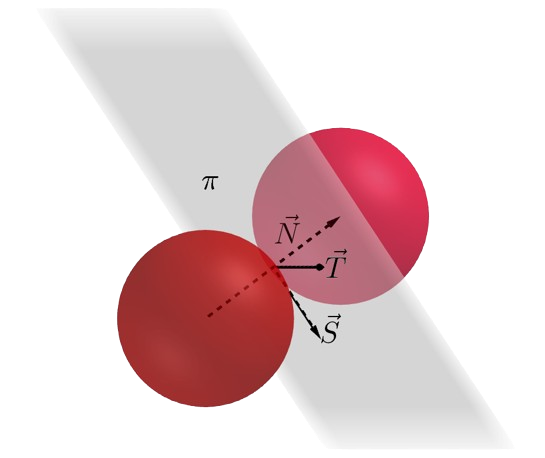
\includegraphics[width=\linewidth]{img/colisao_3d-removebg-preview.png}
        \end{figure}
\end{columns}

\end{frame}

% %------------------------------------------------

% \begin{frame}
% \justifying
% \frametitle{Colisões: Choques elásticos (2/4)}

% \begin{columns}[c]
%     \column{.50\textwidth}\justifying
%         \begin{itemize}
%             \item Energia cinética conservada;
%             \item Momento linear total conservado.
%         \end{itemize}
    
%     \column{.10\textwidth}\justifying
%         \begin{align*}
%             \vet v_1^* &= \vet v_1 + m_2 c_{12} \hat{\vet N},
%             \\
%             \vet v_2^* &= \vet v_2 - m_1 c_{12} \hat{\vet N},
%             \\
%             c_{12} &= \dfrac{2 \langle\vet v_2 - \vet v_1, \hat{\vet N} \rangle}{m_1 + m_2}
%         \end{align*}
    
%     \column{.30\textwidth}\justifying
%         \begin{figure}
%             \centering
%             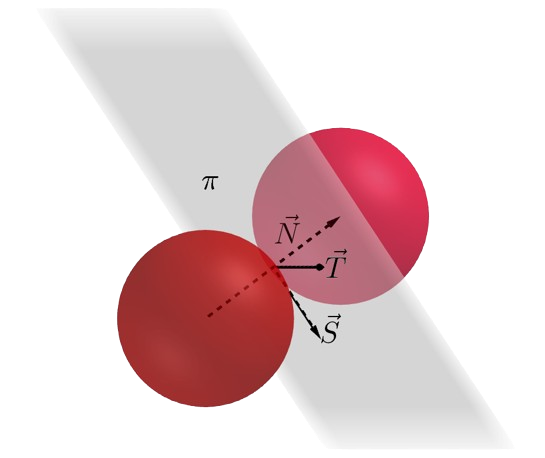
\includegraphics[width=\linewidth]{img/colisao_3d-removebg-preview.png}
%         \end{figure}
% \end{columns}
% \pause
% \begin{alertblock}{Observações}
%     Choques elásticos criam descontinuidades...
% \end{alertblock}

% \end{frame}

% %------------------------------------------------

% \begin{frame}
% \justifying
% \frametitle{Colisões: Potencial amortecido (3/4)}

% \begin{block}{Potencial amortecido}
% Dado um $\varepsilon > 0$, podemos definir
% $$
% V_\varepsilon = - \sum_{a < b} \dfrac{m_a m_b}{\sqrt{\norma{\vet q_b - \vet q_a}^2 + \varepsilon^2}}.
% $$
% \end{block}

% \begin{exampleblock}{}
%     \begin{itemize}
%         \item Potencial correspondente a uma esfera de Plummer.
%         \item Soluções suaves para todo $t$ e qualquer condição inicial.
%     \end{itemize}
% \end{exampleblock}
% \pause
% \begin{alertblock}{}
%     A dinâmica muda! 
% \end{alertblock}

% \end{frame}

% %------------------------------------------------

\begin{frame}
\justifying
\frametitle{Colisões (2/2)}

\begin{exampleblock}{Exemplos}
    Problema IAU-25 via svcp6s9 com $h=10^{-4}$.
    \begin{itemize}
        \item Potencial amortecido com $\varepsilon = 0.1$;
        \item Potencial amortecido com $\varepsilon = 0.05$;
        \item Choques com raio $r=0.1$;
        \item Choques com raio $r=0.05$.
    \end{itemize}
    {\color{blue}\href{https://ime.usp.br/~oapotalej/arquivos/coloquinho2026/iau25.html}{Vídeos dos exemplos.}}
\end{exampleblock}

\end{frame}

%------------------------------------------------

\begin{frame}
\justifying
\frametitle{Valores iniciais (1/2)}

\begin{itemize}
    \item Existem conjuntos de valores iniciais para os quais conhecemos a solução do problema, as \textit{coreografias}.

    \item São úteis numericamente para testar diferentes métodos de integração.

    \item {\color{blue}\href{https://ime.usp.br/~oapotalej/arquivos/coloquinho2026/coreografias.html}{Algumas coreografias.}}
\end{itemize}

\begin{columns}[c]
\column{.32\textwidth}\justifying
    \begin{figure}
        \centering
        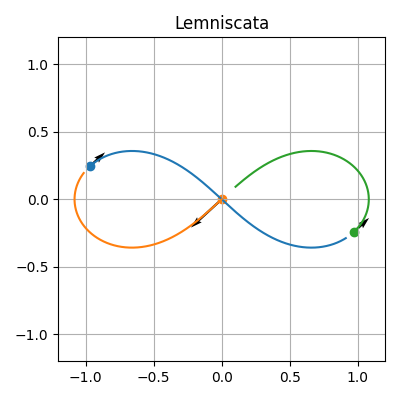
\includegraphics[width=\linewidth]{img/coreografias/lemniscata.png}
    \end{figure}
    
\column{.32\textwidth}\justifying
    \begin{figure}
        \centering
        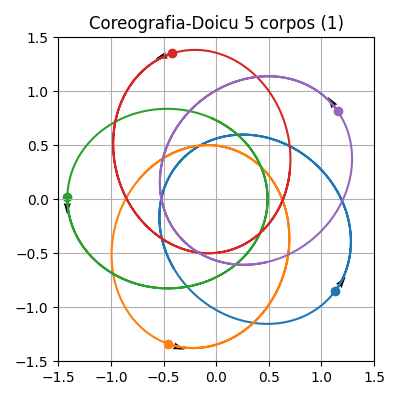
\includegraphics[width=\linewidth]{img/coreografias/ccnmas5_1.png}
    \end{figure}

\column{.32\textwidth}\justifying
    \begin{figure}
        \centering
        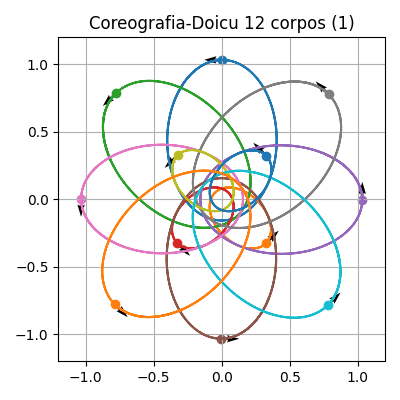
\includegraphics[width=\linewidth]{img/coreografias/ccnmas12_1.png}
    \end{figure}
    
\end{columns}

\end{frame}

%------------------------------------------------

\begin{frame}
\justifying
\frametitle{Sorteando valores iniciais (2/2)}

\begin{columns}
    \column{.60\textwidth}\justifying
        \begin{block}{Ideia}
            Nosso interesse era em problemas com integrais primeiras específicas:
            \begin{enumerate}
                \item Com alguma distribuição, geramos valores iniciais;
                \item Condicionamos os valores gerados para obter as integrais primeiras desejadas.
            \end{enumerate}
        \end{block}
        \pause
        
        \begin{block}{Métodos}
        \begin{itemize}
            \item Iterativo (funciona sempre...).
            \item Direto (necessita potencial homogêneo).
        \end{itemize}

        \href{https://github.com/Potalej/gf-doc-vi}{\textit{Detalhes aqui}}.
        \end{block}

    \column{.40\textwidth}\justifying
        \begin{figure}
            \centering
            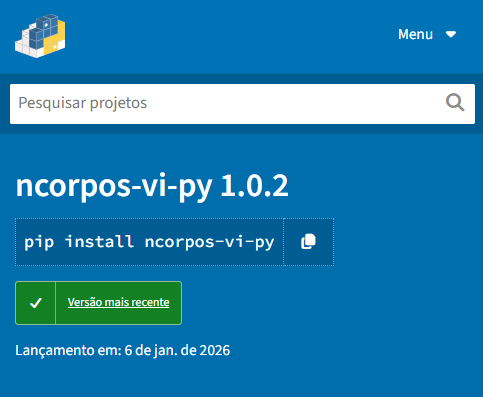
\includegraphics[width=\linewidth]{img/ncorpos_vi_py.png}
            \caption{\href{https://pypi.org/project/ncorpos-vi-py/}{https://pypi.org/project/ncorpos-vi-py/}}
        \end{figure}
\end{columns}

\end{frame}

%------------------------------------------------